\documentclass[12pt, letterpaper]{article}

% --- PAQUETES ---
\usepackage{lmodern}
\usepackage[utf8]{inputenc}
\usepackage[T1]{fontenc}
\usepackage[provide=*, spanish]{babel}
\usepackage[top=2cm, bottom=2cm, left=2cm, right=2cm]{geometry}
\usepackage{graphicx}
\usepackage[table]{xcolor}
\usepackage{enumitem}
\usepackage{amssymb}
\usepackage{amsmath}
\usepackage{multicol}
\usepackage{helvet}
\usepackage{pifont}
\usepackage{fontawesome5}
\usepackage{array}
\usepackage{cancel}
\usepackage{longtable}
\usepackage{tikz}
\usepackage{comment}
\usetikzlibrary{
	arrows.meta, shapes.geometric, positioning, calc,
	decorations.pathmorphing, backgrounds, fit, shadows.blur, patterns
}

% --- COLORES (paleta oficial del Liceo V.A.L.) ---
\definecolor{valblue}       {RGB}{0,   74,  153}
\definecolor{valgreen}      {RGB}{0,  153,   76}
\definecolor{valred}        {RGB}{204,   0,    0}
\definecolor{valdark}       {RGB}{ 30,  30,   30}
\definecolor{valorange}     {RGB}{230, 115,    0}
\definecolor{vallightblue}  {RGB}{220, 235,  255}
\definecolor{vallightgreen} {RGB}{220, 255,  235}
\definecolor{vallightred}   {RGB}{255, 220,  220}
\definecolor{vallightorange}{RGB}{255, 240,  215}
\definecolor{valgray}       {RGB}{248, 248,  248}
\definecolor{valmid}        {RGB}{190, 190,  190}
\definecolor{boxbg}         {RGB}{245, 245,  245}
\definecolor{valpurple}     {RGB}{111,  56,  156}
\definecolor{vallightpurple}{RGB}{235, 224,  245}

\renewcommand{\familydefault}{\sfdefault}

\usepackage[most]{tcolorbox}
\usepackage{eso-pic}
\AddToShipoutPictureBG{%
	\AtPageLowerLeft{%
		
\includegraphics[width=\paperwidth,height=\paperheight,
		keepaspectratio=false]{../../FondoVAL.pdf}}}

% --- ENTORNOS INSTITUCIONALES (idénticos a U6M14/U6M-13) ---
\newtcolorbox{concepto}[1]{breakable, colback=valblue!5,
	colframe=valblue,
	title={\ding{111}\ \textbf{Aprende el Concepto: #1}},
	arc=2mm, boxrule=1pt, fonttitle=\large}
\newtcolorbox{truco}[1]{breakable, colback=valorange!5,
	colframe=valorange,
	title={\ding{51}\;\textbf{El Truco: #1}},
	arc=2mm, boxrule=1pt, fonttitle=\large}
\newtcolorbox{ejemplo}{breakable, colback=valgreen!5,
	colframe=valgreen,
	title={\ding{45}\;\textbf{Ejemplo}},
	arc=2mm, boxrule=1pt}
\newtcolorbox{atencion}[1]{breakable, colback=vallightred,
	colframe=valred,
	title={\textbf{\color{white}#1}},
	attach boxed title to top left={yshift=-2.5mm, xshift=5mm},
	boxed title style={colback=valred, sharp corners},
	arc=2mm, boxrule=1pt}
\newenvironment{practica}[1]{%
	\vspace{0.4cm}
	\noindent{\Large\textbf{\textcolor{valblue}{\ding{46}\;¡Tu Turno! (#1)}}}
	\vspace{0.1cm}\hrule\vspace{0.3cm}}{\vspace{0.3cm}}
\newtcolorbox{espaciotrabajo}[1]{colback=white,
	colframe=valdark!40,
	title={\small\textbf{Procedimiento: #1}},
	arc=1mm, boxrule=0.6pt, coltitle=valdark!90,
	top=2mm, bottom=2mm}
\newtcolorbox{espaciotrabajonb}[1]{colback=white,
	colframe=valdark!40,
	title={\small\textbf{Procedimiento: #1}},
	arc=1mm, boxrule=0.6pt, coltitle=valdark!90,
	top=2mm, bottom=2mm}

% --- CASILLAS (idénticas) ---
\newcommand{\boxfill}[1][1.5cm]{\tcbox[on line, size=minimal,
	colframe=valdark!60, colback=boxbg, boxrule=0.8pt, arc=1mm,
	boxsep=3pt, left=2pt, right=2pt, top=2pt, bottom=2pt]%
	{\makebox[#1]{\vphantom{M}}}}
\newcommand{\boxstep}[1][2cm]{\tcbox[on line, size=minimal,
	colframe=valdark!40, colback=white, boxrule=0.8pt, arc=1mm,
	boxsep=3pt, left=2pt, right=2pt, top=2pt, bottom=2pt]%
	{\makebox[#1]{\vphantom{M}}}}

\setlength{\columnseprule}{0.4pt}

% --- CAJAS EXTRA PARA EJEMPLOS (idénticas) ---
\newtcolorbox{pasocaja}[3]{
	enhanced, colback=#1!8, colframe=#1,
	title={\textbf{Paso #2:} #3},
	arc=2mm, boxrule=1.2pt, fonttitle=\normalsize,
	left=4pt, right=4pt, top=3pt, bottom=3pt,
	attach boxed title to top left={yshift=-2mm, xshift=4mm},
	boxed title style={colback=#1, arc=1.5mm, sharp corners=south}}

\newtcolorbox{ejemploresuelto}[1]{
	breakable, enhanced,
	colback=valgreen!4, colframe=valgreen,
	title={\faCalculator\;\textbf{Ejemplo: #1}},
	arc=3mm, boxrule=1.5pt, fonttitle=\large,
	attach boxed title to top left={yshift=-3mm, xshift=6mm},
	boxed title style={colback=valgreen, arc=2mm}}

\newtcolorbox{minicheck}{
	breakable,
	colback=valorange!8, colframe=valorange,
	title={\ding{51}\;\textbf{Comprueba tú mismo antes de continuar}},
	arc=2mm, boxrule=1pt, fonttitle=\normalsize}

\newtcolorbox{errorcomun}[1]{
	colback=vallightred, colframe=valred,
	title={\faExclamationTriangle\;\textbf{Error Frecuente: #1}},
	arc=2mm, boxrule=1pt, fonttitle=\normalsize}

% --- ENTORNO: DEMOSTRACIÓN GEOMÉTRICA (prueba formal y completa de cada fórmula) ---
\newtcolorbox{demostracion}[1]{
	breakable, enhanced,
	colback=valpurple!5, colframe=valpurple,
	title={\ding{228}\;\textbf{Demostración: #1}},
	arc=2mm, boxrule=1.2pt, fonttitle=\large,
	attach boxed title to top left={yshift=-2.7mm, xshift=5mm},
	boxed title style={colback=valpurple, arc=1.5mm, sharp corners=south}}

% ============================================================
\begin{document}
	% ============================================================
	
	% ─────────────────────────────────────────────────────────────
	% PORTADA
	% ─────────────────────────────────────────────────────────────
	\begin{center}
		{\Huge\textbf{LICEO V.A.L.}}\\[0.5cm]
		{\LARGE\textbf{MÓDULO DE AUTOAPRENDIZAJE}}\\[0.5cm]
		{\Large\textbf{MATEMÁTICAS 6$^\circ$}}\\[0.5cm]
		\begin{tcolorbox}[colback=valblue!10, colframe=valblue,
			arc=3mm, boxrule=1.5pt]
			\centering
			\Huge\textbf{UNIDAD 16}\\[0.25cm]
			\Large\textbf{Perímetros y Áreas, Rectas ($\perp$, $\parallel$)}\\[0.1cm]
			\Large\textbf{y Transformaciones Geométricas}\\[0.2cm]
			\large Área y perímetro de polígonos, rectas notables y transformaciones en el plano.
		\end{tcolorbox}
		\vspace{0.6cm}
		\begin{tcolorbox}[colback=white, colframe=valblue,
			width=12cm, arc=3mm, boxrule=1.5pt]
			\centering\vspace{0.3cm}
			\textbf{Nombre:}\\[0.3cm]
			\underline{\hspace{9cm}}\\[0.5cm]
			\textbf{Código:}\;\underline{06M-16 FL}
			\hspace{1cm}\textbf{Año:}\;\underline{2026}
			\vspace{0.3cm}
		\end{tcolorbox}
		\vspace{0.8cm}
		\textit{``Hacia un Aprendizaje Significativo, Autónomo y en Libertad''}
	\end{center}
	
	% =========================================================
	%  MISIÓN 1 — ÁREA Y PERÍMETRO DE POLÍGONOS
	% =========================================================
	\section*{Misión 1: Área y Perímetro de Polígonos}
	
	\begin{concepto}{Ideas de Base}
		\textbf{Perímetro (P):} suma de las longitudes de \textbf{todos} los lados de una figura. Se mide en unidades de \textbf{longitud} (cm, m, km\ldots).\\
		\textbf{Área (A):} medida de la superficie \textbf{encerrada} por una figura. Se mide en unidades \textbf{cuadradas} (cm$^2$, m$^2$\ldots).
		
		\vspace{0.3cm}
		Desde grados anteriores ya sabes que, para un \textbf{rectángulo} de base $b$ y altura $h$:
		$$P_{\text{rect}} = 2b + 2h \qquad\qquad A_{\text{rect}} = b \times h$$
		
		\begin{center}
			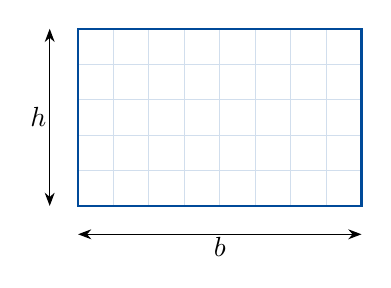
\begin{tikzpicture}[scale=0.9]
				\draw[step=0.5,valblue!18,thin] (0,0) grid (4,2.5);
				\draw[thick,valblue] (0,0) rectangle (4,2.5);
				\draw[{Stealth}-{Stealth}] (0,-0.4)--(4,-0.4) node[midway,below,fill=white,inner sep=1pt] {$b$};
				\draw[{Stealth}-{Stealth}] (-0.4,0)--(-0.4,2.5) node[midway,left,fill=white,inner sep=1pt] {$h$};
			\end{tikzpicture}
		\end{center}
		Estas dos ideas son la \textbf{base} de toda la misión: cada nueva fórmula que verás compara una figura con un rectángulo o un paralelogramo.
	\end{concepto}
	
	\begin{concepto}{Área del Triángulo}
		Para cualquier triángulo de base $b$ y altura $h$ (el segmento \textbf{perpendicular}, ángulo de $90^\circ$, desde un vértice hasta la recta que contiene el lado opuesto):
		$$A_{\triangle} = \dfrac{b \times h}{2}$$
		
		\begin{center}
			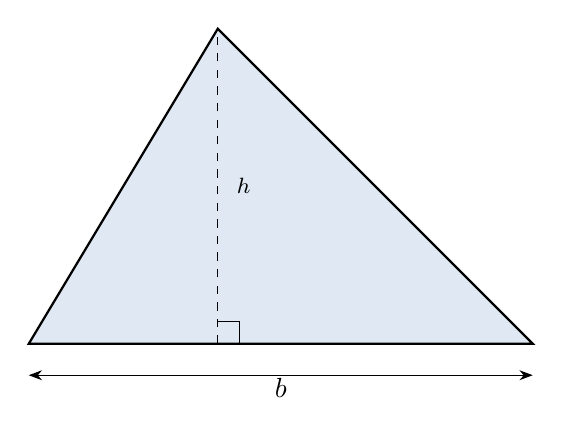
\begin{tikzpicture}[scale=0.8]
				\draw[thick,fill=valblue!12] (0,0)--(8,0)--(3,5)--cycle;
				\draw[dashed] (3,0)--(3,5);
				\draw (3,0.35)--(3.35,0.35)--(3.35,0);
				\draw[{Stealth}-{Stealth}] (0,-0.5)--(8,-0.5) node[midway,below,fill=white,inner sep=1pt] {$b$};
				\node[right] at (3.15,2.5) {\footnotesize $h$};
			\end{tikzpicture}
		\end{center}
	\end{concepto}
	
	\begin{comment}
		
	
	\begin{demostracion}{Área del Triángulo}
		\textbf{Caso 1 — triángulo rectángulo (la altura coincide con un lado).}
		Todo rectángulo de base $b$ y altura $h$ queda dividido por su diagonal en \textbf{dos triángulos rectángulos exactamente congruentes} (mismos tres lados, criterio LLL). El área del rectángulo es $b\times h$; como los dos triángulos son iguales y la cubren por completo, cada uno tiene la mitad:
		$$A_{\triangle} = \frac{b\times h}{2}$$
		
		\begin{center}
			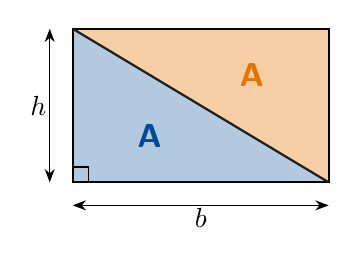
\begin{tikzpicture}[scale=0.65]
				\fill[valblue!30] (0,0) -- (0,3) -- (5,0) -- cycle;
				\fill[valorange!35] (0,3) -- (5,3) -- (5,0) -- cycle;
				\draw[thick] (0,0) rectangle (5,3);
				\draw[thick,valdark] (0,3) -- (5,0);
				\draw (0,0.3)--(0.3,0.3)--(0.3,0);
				\draw[{Stealth}-{Stealth}] (0,-0.45)--(5,-0.45) node[midway,below,fill=white,inner sep=1pt] {$b$};
				\draw[{Stealth}-{Stealth}] (-0.45,0)--(-0.45,3) node[midway,left,fill=white,inner sep=1pt] {$h$};
				\node[valblue,font=\bfseries\large] at (1.5,0.9) {A};
				\node[valorange,font=\bfseries\large] at (3.5,2.1) {A};
			\end{tikzpicture}
		\end{center}
		
		\textbf{Caso 2 — triángulo cualquiera (acutángulo), el pie de la altura cae dentro de la base.}
		Al trazar la altura desde el vértice $A$ hasta el punto $H$ sobre $BC$, el triángulo $ABC$ queda partido en dos triángulos rectángulos: $ABH$ (base $m$, altura $h$) y $AHC$ (base $n$, altura $h$), con $m+n=b$.
		$$A_{ABH}=\frac{m\times h}{2} \qquad A_{AHC}=\frac{n\times h}{2}$$
		$$A_{ABC}=A_{ABH}+A_{AHC}=\frac{m\times h}{2}+\frac{n\times h}{2}=\frac{(m+n)\times h}{2}=\frac{b\times h}{2}$$
		
		\begin{center}
			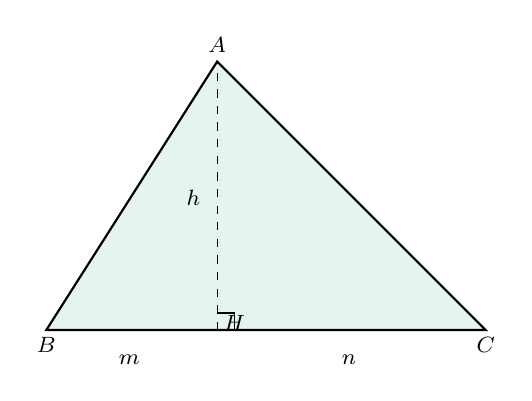
\begin{tikzpicture}[scale=0.62]
				\draw[thick,fill=valgreen!10] (0,0)--(9,0)--(3.5,5.5)--cycle;
				\draw[dashed] (3.5,0)--(3.5,5.5);
				\draw (3.5,0.35)--(3.85,0.35)--(3.85,0);
				\node[below] at (1.7,-0.3) {\footnotesize $m$};
				\node[below] at (6.2,-0.3) {\footnotesize $n$};
				\node[left] at (3.35,2.7) {\footnotesize $h$};
				\node at (0,-0.3) {\footnotesize $B$};
				\node at (9,-0.3) {\footnotesize $C$};
				\node at (3.5,5.85) {\footnotesize $A$};
				\node at (3.85,0.15) {\footnotesize $H$};
			\end{tikzpicture}
		\end{center}
		
		\begin{atencion}{Nota: ¿y si el triángulo es obtusángulo?}
			Si el ángulo en $B$ o en $C$ es obtuso, el pie de la altura $H$ cae \textbf{fuera} del segmento $BC$ (sobre su prolongación). En ese caso $A_{ABC}=A_{AHC}-A_{ABH}$ (una resta en vez de una suma), y al simplificar se obtiene exactamente la \textbf{misma} fórmula $A=\dfrac{b\times h}{2}$. La fórmula funciona siempre, sin importar el tipo de triángulo.
		\end{atencion}
	\end{demostracion}
\end{comment}

	\begin{concepto}{Área del Trapecio}
		Un trapecio tiene dos lados \textbf{paralelos} llamados \textbf{bases}: la base mayor $b_1$ y la base menor $b_2$; y una \textbf{altura} $h$ (distancia perpendicular entre las dos bases). Su área es:
		$$A_{\text{trapecio}} = \dfrac{(b_1+b_2)\times h}{2}$$
		
		\begin{center}
			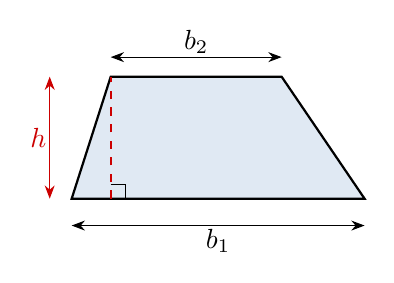
\begin{tikzpicture}[scale=0.62]
				\draw[thick,fill=valblue!12] (0,0) -- (6,0) -- (4.3,2.5) -- (0.8,2.5) -- cycle;
				\draw[dashed,valred,thick] (0.8,0)--(0.8,2.5);
				\draw (0.8,0.3)--(1.1,0.3)--(1.1,0);
				\draw[{Stealth}-{Stealth}] (0,-0.55)--(6,-0.55) node[midway,below,fill=white,inner sep=1pt] {$b_1$};
				\draw[{Stealth}-{Stealth}] (0.8,2.9)--(4.3,2.9) node[midway,above,fill=white,inner sep=1pt] {$b_2$};
				\draw[{Stealth}-{Stealth},valred] (-0.45,0)--(-0.45,2.5) node[midway,left,fill=white,inner sep=1pt] {$h$};
			\end{tikzpicture}
		\end{center}
	\end{concepto}
	
	\begin{comment}
	
	\begin{demostracion}{Área del Trapecio}
		Tomamos una \textbf{copia idéntica} del trapecio, la \textbf{giramos $180^\circ$} y la unimos al original por uno de sus lados inclinados:
		
		\begin{center}
			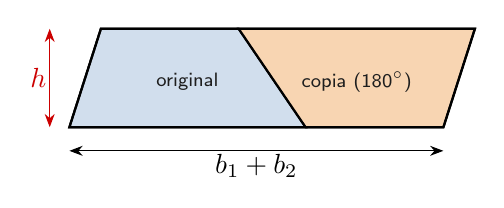
\begin{tikzpicture}[scale=0.5]
				\draw[thick,fill=valblue!18] (0,0)--(6,0)--(4.3,2.5)--(0.8,2.5)--cycle;
				\draw[thick,fill=valorange!30] (6,0)--(9.5,0)--(10.3,2.5)--(4.3,2.5)--cycle;
				\draw[thick] (0,0)--(9.5,0)--(10.3,2.5)--(0.8,2.5)--cycle;
				\draw[{Stealth}-{Stealth}] (0,-0.6)--(9.5,-0.6) node[midway,below,fill=white,inner sep=1pt] {$b_1+b_2$};
				\draw[{Stealth}-{Stealth},valred] (-0.5,0)--(-0.5,2.5) node[midway,left,fill=white,inner sep=1pt] {$h$};
				\node[font=\scriptsize,valdark] at (3,1.15) {original};
				\node[font=\scriptsize,valdark] at (7.3,1.15) {copia (180$^\circ$)};
			\end{tikzpicture}
		\end{center}
		
		La base mayor de un trapecio queda pegada a la base menor del otro, así que la figura nueva es un \textbf{paralelogramo} cuya base mide $b_1+b_2$ y cuya altura sigue siendo $h$ (la copia girada no cambia la separación entre las bases). Como el área de un paralelogramo es (base)$\times$(altura):
		$$A_{\text{paralelogramo}} = (b_1+b_2)\times h$$
		Ese paralelogramo está formado por \textbf{dos} trapecios congruentes (el original y su copia), así que el área de \textbf{uno solo} es la mitad:
		$$A_{\text{trapecio}} = \dfrac{(b_1+b_2)\times h}{2}$$
	\end{demostracion}
	
	
	\begin{truco}{Todas las Fórmulas Están Conectadas}
		Si en la fórmula del trapecio haces que $b_2$ valga \textbf{cero}, el trapecio se convierte en un \textbf{triángulo}:
		$$A = \dfrac{(b_1+0)\times h}{2} = \dfrac{b_1 \times h}{2}$$
		¡Es la misma fórmula del triángulo! El triángulo es, en el fondo, un ``trapecio especial'' donde una base se redujo a un punto. Más adelante verás que el polígono regular también se reduce a esta misma idea: \textbf{todo se construye a partir de triángulos}.
		
		\vspace{0.2cm}
		\textbf{Atajo de cálculo mental:} en el trapecio, suma primero $b_1+b_2$ y verifica si ese resultado simplifica bien con la altura. Divide entre 2 \textbf{una sola vez}, al final de toda la operación.
	\end{truco}
\end{comment}
	\begin{concepto}{Área y Perímetro de Polígonos Regulares}
		Un polígono es \textbf{regular} cuando todos sus lados son congruentes \textbf{y} todos sus ángulos internos son congruentes (ej.: triángulo equilátero, cuadrado, pentágono regular, hexágono regular\ldots).
		
		\vspace{0.2cm}
		Dos elementos nuevos:
		\begin{itemize}
			\item \textbf{Lado ($s$):} longitud de cada lado (todos miden igual).
			\item \textbf{Apotema ($a$):} distancia \textbf{perpendicular} desde el centro del polígono hasta el punto medio de un lado.
		\end{itemize}
		
		Si el polígono tiene $n$ lados:
		$$P = n \times s \qquad\qquad A_{\text{polígono regular}} = \dfrac{P \times a}{2}$$
		
		\begin{center}
			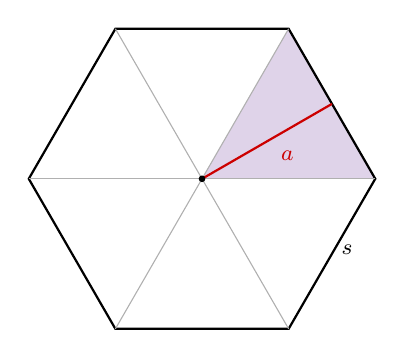
\begin{tikzpicture}[scale=0.55]
				\foreach \i in {0,...,5}{\coordinate (P\i) at ({60*\i}:4);}
				\fill[valpurple!22] (0,0)--(P0)--(P1)--cycle;
				\draw[thick] (P0)--(P1)--(P2)--(P3)--(P4)--(P5)--cycle;
				\foreach \i in {0,...,5}{\draw[valdark!35] (0,0)--(P\i);}
				\draw[thick,valred] (0,0)--(3,1.73);
				%\draw (2.55,0.66)--(2.75,1.02)--(2.4,1.22);
				\fill (0,0) circle (2.2pt);
				\node[valred,below right] at (1.6,0.87) {\footnotesize $a$};
				\node[below right] at (3,-1.3) {\footnotesize $s$};
			\end{tikzpicture}
		\end{center}
	\end{concepto}
	
	\begin{comment}
		
	
	\begin{demostracion}{Área del Polígono Regular}
		Desde el centro, se trazan segmentos a \textbf{cada uno} de los $n$ vértices. Esto divide el polígono en $n$ triángulos \textbf{congruentes} entre sí, cada uno con base $s$ (un lado del polígono) y altura $a$ (la apotema, pues el segmento del centro al punto medio del lado es perpendicular a ese lado).
		
		Cada triángulo tiene área $\dfrac{s\times a}{2}$. Como hay $n$ triángulos iguales:
		$$A_{\text{polígono}} = n\times \dfrac{s\times a}{2} = \dfrac{(n\times s)\times a}{2}$$
		Pero $n\times s$ es exactamente el \textbf{perímetro} $P$ del polígono (son los $n$ lados sumados). Sustituyendo:
		$$A_{\text{polígono regular}} = \dfrac{P\times a}{2}$$
		Esta es la misma idea del triángulo y el trapecio: \textbf{el área siempre se construye repartiendo la figura en triángulos.}
	\end{demostracion}
\end{comment}

	\begin{ejemploresuelto}{Área y Perímetro de un Triángulo}
		\textbf{Situación:} un triángulo tiene base $b=14$ cm y altura $h=9$ cm.
		\begin{center}
			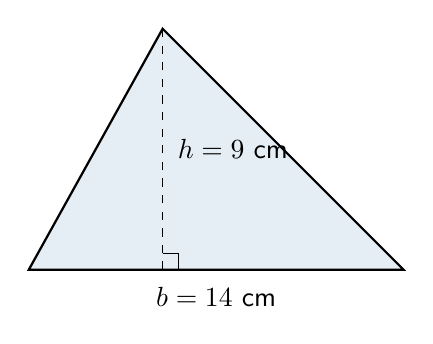
\begin{tikzpicture}[scale=0.34]
				\draw[thick,fill=valblue!10] (0,0)--(14,0)--(5,9)--cycle;
				\draw[dashed] (5,0)--(5,9);
				\draw (5,0.6)--(5.6,0.6)--(5.6,0);
				\node[below] at (7,-0.3) {$b=14$ cm};
				\node[right] at (5.2,4.5) {$h=9$ cm};
			\end{tikzpicture}
		\end{center}
		\begin{pasocaja}{valblue}{1}{Identificar los datos}
			\centering Base $b=14$ cm \qquad Altura $h=9$ cm
		\end{pasocaja}
		\begin{pasocaja}{valgreen}{2}{Aplicar la fórmula}
			\centering $A_{\triangle} = \dfrac{b \times h}{2} = \dfrac{14 \times 9}{2} = \dfrac{126}{2}$
		\end{pasocaja}
		\begin{pasocaja}{valorange}{3}{Resultado}
			\centering $A = \mathbf{63\ cm^2}$ \quad (el perímetro no se puede hallar: faltan los otros dos lados).
		\end{pasocaja}
	\end{ejemploresuelto}
	
	\begin{ejemploresuelto}{Área y Perímetro de un Trapecio}
		\textbf{Situación:} base mayor $b_1=16$ cm, base menor $b_2=10$ cm, altura $h=4$ cm, lados no paralelos de $5$ cm cada uno.
		\begin{center}
			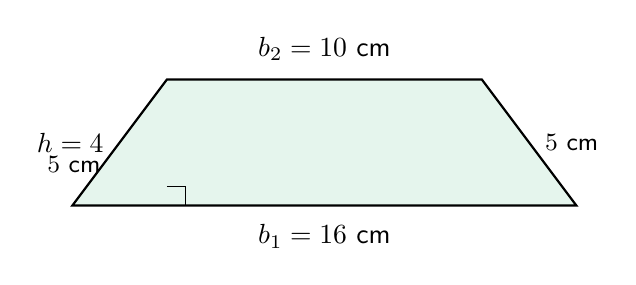
\begin{tikzpicture}[scale=0.4]
				\draw[thick,fill=valgreen!10] (0,0)--(16,0)--(13,4)--(3,4)--cycle;
				\draw (3,0.6)--(3.6,0.6)--(3.6,0);
				\node[below] at (8,-0.3) {$b_1=16$ cm};
				\node[above] at (8,4.3) {$b_2=10$ cm};
				\node[left] at (1.3,2) {$h=4$};
				\node[right] at (14.7,2) {\small $5$ cm};
				\node[left] at (1.2,1.3) {\small $5$ cm};
			\end{tikzpicture}
		\end{center}
		\begin{pasocaja}{valblue}{1}{Identificar los datos}
			\centering $b_1=16$ cm \quad $b_2=10$ cm \quad $h=4$ cm \quad lados $=5$ cm y $5$ cm
		\end{pasocaja}
		\begin{pasocaja}{valgreen}{2}{Área}
			\centering $A = \dfrac{(b_1+b_2)\times h}{2} = \dfrac{(16+10)\times 4}{2} = \dfrac{26\times 4}{2}=\dfrac{104}{2}$
		\end{pasocaja}
		\begin{pasocaja}{valorange}{3}{Perímetro}
			\centering $P = b_1+b_2+\text{lado}_1+\text{lado}_2 = 16+10+5+5$
		\end{pasocaja}
		\begin{pasocaja}{valdark}{4}{Resultados}
			\centering $A = \mathbf{52\ cm^2} \qquad\qquad P = \mathbf{36\ cm}$
		\end{pasocaja}
	\end{ejemploresuelto}
	
	\begin{ejemploresuelto}{Área y Perímetro de un Polígono Regular}
		\textbf{Situación:} un hexágono regular tiene lado $s=6$ cm y apotema $a=5,2$ cm.
		\begin{center}
			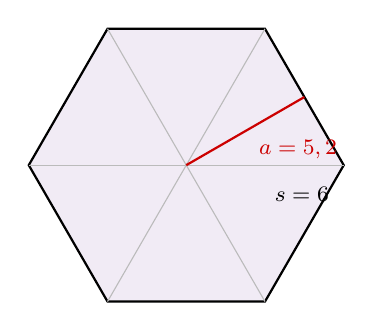
\begin{tikzpicture}[scale=0.5]
				\foreach \i in {0,...,5}{\coordinate (Q\i) at ({60*\i}:4);}
				\draw[thick,fill=valpurple!10] (Q0)--(Q1)--(Q2)--(Q3)--(Q4)--(Q5)--cycle;
				\foreach \i in {0,...,5}{\draw[valdark!30] (0,0)--(Q\i);}
				\node[below right] at (2,-0.3) {\footnotesize $s=6$};
				\draw[valred,thick] (0,0)--(3,1.73);
				\node[valred,below right] at (1.6,0.87) {\footnotesize $a=5,2$};
			\end{tikzpicture}
		\end{center}
		\begin{pasocaja}{valblue}{1}{Perímetro: $n\times s$ (el hexágono tiene $n=6$ lados)}
			\centering $P = 6 \times 6 = 36$ cm
		\end{pasocaja}
		\begin{pasocaja}{valgreen}{2}{Área: $\dfrac{P\times a}{2}$}
			\centering $A = \dfrac{36 \times 5,2}{2} = \dfrac{187,2}{2}$
		\end{pasocaja}
		\begin{pasocaja}{valorange}{3}{Resultados}
			\centering $P = \mathbf{36\ cm} \qquad\qquad A = \mathbf{93,6\ cm^2}$
		\end{pasocaja}
	\end{ejemploresuelto}
	
	\begin{minicheck}
		Sin mirar atrás, escribe de memoria las tres fórmulas de esta misión:
		$$A_{\triangle} = \text{\boxfill[2.6cm]}$$
		$$A_{\text{trapecio}} = \text{\boxfill[3.2cm]}$$
		$$A_{\text{polígono regular}} = \text{\boxfill[2.8cm]}$$
		Un triángulo tiene $b=20$ cm y $h=7$ cm. Su área es \boxfill[2.2cm]. Un pentágono regular tiene $P=40$ cm y $a=5,5$ cm. Su área es \boxfill[2.2cm]
	\end{minicheck}
	
	\begin{practica}{Área y Perímetro de Polígonos}
		
		\textbf{A) Cálculo directo: extrae los datos de cada gráfica y opera.}
		
		\begin{multicols}{2}
			\begin{enumerate}[label=\textbf{\arabic*.}, itemsep=0.7cm]
				\item Halla el \textbf{área}.
				\begin{center}
					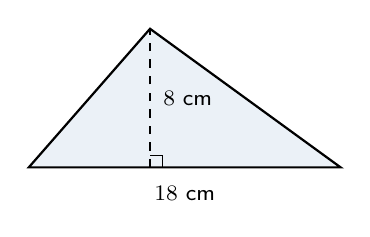
\begin{tikzpicture}[scale=0.22]
						\draw[thick,fill=valblue!8] (0,0)--(18,0)--(7,8)--cycle;
						\draw[dashed] (7,0)--(7,8);
						\draw (7,0.7)--(7.7,0.7)--(7.7,0);
						\node[below] at (9,-0.5) {\footnotesize $18$ cm};
						\node[right] at (7.2,4) {\footnotesize $8$ cm};
					\end{tikzpicture}
				\end{center}
				$A=\dfrac{\boxfill[1.1cm]\times\boxfill[1.1cm]}{\boxfill[0.6cm]}=$\boxfill[1.6cm]
				
				\item Halla el \textbf{área} y el \textbf{perímetro}.
				\begin{center}
					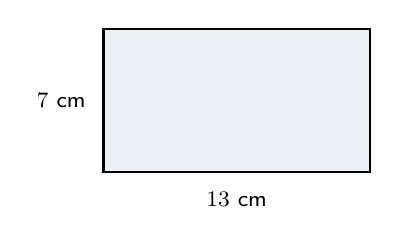
\begin{tikzpicture}[scale=0.26]
						\draw[thick,fill=valblue!8] (0,0) rectangle (13,7);
						\node[below] at (6.5,-0.5) {\footnotesize $13$ cm};
						\node[left] at (-0.4,3.5) {\footnotesize $7$ cm};
					\end{tikzpicture}
				\end{center}
				$A=\boxfill[1cm]\times\boxfill[1cm]=$\boxfill[1.4cm]\\
				$P=2(\boxfill[0.7cm]+\boxfill[0.7cm])=$\boxfill[1.3cm]
				
				\item Halla el \textbf{área}.
				\begin{center}
					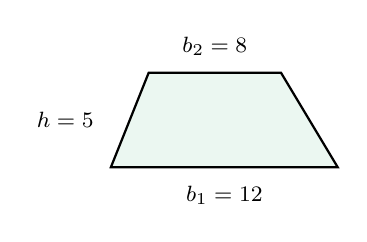
\begin{tikzpicture}[scale=0.24]
						\draw[thick,fill=valgreen!8] (0,0)--(12,0)--(9,5)--(2,5)--cycle;
						\node[below] at (6,-0.5) {\footnotesize $b_1=12$};
						\node[above] at (5.5,5.4) {\footnotesize $b_2=8$};
						\node[left] at (-0.4,2.5) {\footnotesize $h=5$};
					\end{tikzpicture}
				\end{center}
				$A=\dfrac{(\boxfill[0.7cm]+\boxfill[0.7cm])\times\boxfill[0.7cm]}{\boxfill[0.5cm]}=$\boxfill[1.3cm]
				
				\item Halla el \textbf{área} y el \textbf{perímetro}.
				\begin{center}
					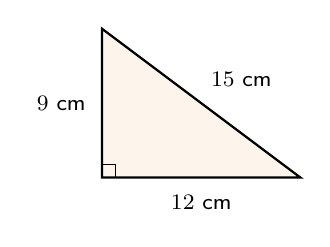
\begin{tikzpicture}[scale=0.21]
						\draw[thick,fill=valorange!8] (0,0)--(12,0)--(0,9)--cycle;
						\draw (0,0.8)--(0.8,0.8)--(0.8,0);
						\node[below] at (6,-0.5) {\footnotesize $12$ cm};
						\node[left] at (-0.4,4.5) {\footnotesize $9$ cm};
						\node[above right] at (6,4.9) {\footnotesize $15$ cm};
					\end{tikzpicture}
				\end{center}
				$A=\dfrac{\boxfill[1.1cm]\times\boxfill[1.1cm]}{\boxfill[0.6cm]}=$\boxfill[1.6cm]\\
				$P=\boxfill[0.8cm]+\boxfill[0.8cm]+\boxfill[0.8cm]=$\boxfill[1.6cm]
				
				\item Halla el \textbf{área} y el \textbf{perímetro}.
				\begin{center}
					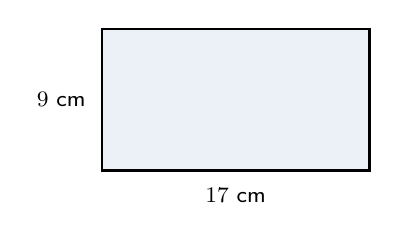
\begin{tikzpicture}[scale=0.2]
						\draw[thick,fill=valblue!8] (0,0) rectangle (17,9);
						\node[below] at (8.5,-0.5) {\footnotesize $17$ cm};
						\node[left] at (-0.4,4.5) {\footnotesize $9$ cm};
					\end{tikzpicture}
				\end{center}
				$A=\boxfill[1cm]\times\boxfill[1cm]=$\boxfill[1.4cm]\\
				$P=2(\boxfill[0.7cm]+\boxfill[0.7cm])=$\boxfill[1.3cm]
				
				\item Halla el \textbf{área} y el \textbf{perímetro} (trapecio isósceles).
				\begin{center}
					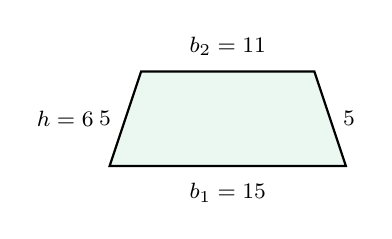
\begin{tikzpicture}[scale=0.2]
						\draw[thick,fill=valgreen!8] (0,0)--(15,0)--(13,6)--(2,6)--cycle;
						\node[below] at (7.5,-0.5) {\footnotesize $b_1=15$};
						\node[above] at (7.5,6.4) {\footnotesize $b_2=11$};
						\node[left] at (-0.4,3) {\footnotesize $h=6$};
						\node[right] at (14.2,3) {\footnotesize $5$};
						\node[left] at (0.7,3) {\footnotesize $5$};
					\end{tikzpicture}
				\end{center}
				$A=\dfrac{(\boxfill[0.7cm]+\boxfill[0.7cm])\times\boxfill[0.7cm]}{\boxfill[0.5cm]}=$\boxfill[1.3cm]\\
				$P=$\boxfill[3.2cm]$=$\boxfill[1.4cm]
				
				\item Halla el \textbf{área} y el \textbf{perímetro}.
				\begin{center}
					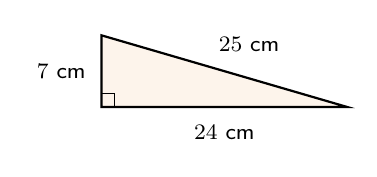
\begin{tikzpicture}[scale=0.13]
						\draw[thick,fill=valorange!8] (0,0)--(24,0)--(0,7)--cycle;
						\draw (0,1.3)--(1.3,1.3)--(1.3,0);
						\node[below] at (12,-0.8) {\footnotesize $24$ cm};
						\node[left] at (-0.6,3.5) {\footnotesize $7$ cm};
						\node[above right] at (10.5,4.5) {\footnotesize $25$ cm};
					\end{tikzpicture}
				\end{center}
				$A=\dfrac{\boxfill[1.1cm]\times\boxfill[1.1cm]}{\boxfill[0.6cm]}=$\boxfill[1.6cm]\\
				$P=\boxfill[0.8cm]+\boxfill[0.8cm]+\boxfill[0.8cm]=$\boxfill[1.6cm]
				
				\item Halla el \textbf{área} y el \textbf{perímetro} (cuidado: hay decimales).
				\begin{center}
					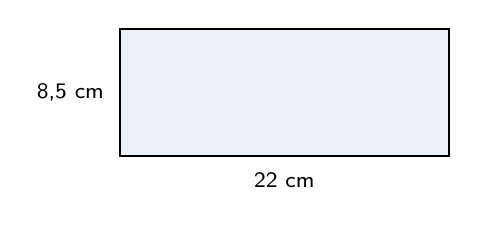
\begin{tikzpicture}[scale=0.19]
						\draw[thick,fill=valblue!8] (0,0) rectangle (22,8.5);
						\node[below] at (11,-0.5) {\footnotesize 22 cm};
						\node[left] at (-0.4,4.25) {\footnotesize 8,5 cm};
					\end{tikzpicture}
				\end{center}
				$A=\boxfill[1cm]\times\boxfill[1cm]=$\boxfill[1.4cm]\\
				$P=2(\boxfill[0.7cm]+\boxfill[0.7cm])=$\boxfill[1.3cm]
				
				\item Halla el \textbf{área} (pista: suma las bases primero).
				\begin{center}
					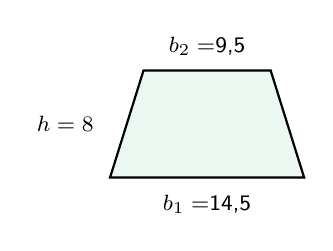
\begin{tikzpicture}[scale=0.17]
						\draw[thick,fill=valgreen!8] (0,0)--(14.5,0)--(12,8)--(2.5,8)--cycle;
						\node[below] at (7.25,-0.6) {\footnotesize $b_1=$14,5};
						\node[above] at (7.25,8.4) {\footnotesize $b_2=$9,5};
						\node[left] at (-0.5,4) {\footnotesize $h=8$};
					\end{tikzpicture}
				\end{center}
				$A=\dfrac{(\boxfill[0.7cm]+\boxfill[0.7cm])\times\boxfill[0.7cm]}{\boxfill[0.5cm]}=$\boxfill[1.3cm]
			\end{enumerate}
		\end{multicols}
		
		\vspace{0.3cm}
		\textbf{B) Problemas aplicados: extrae las medidas de la gráfica y resuelve la situación.}
		
		\begin{multicols}{2}
			\begin{enumerate}[label=\textbf{\arabic*.}, itemsep=1cm, start=10]
				\item \textbf{Jardinería.} Un jardín rectangular tiene las medidas de la gráfica. Se necesita saber cuánto césped comprar (área) y cuánta cerca poner alrededor (perímetro).
				\begin{center}
					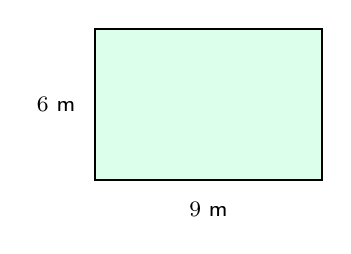
\begin{tikzpicture}[scale=0.32]
						\draw[thick,fill=vallightgreen] (0,0) rectangle (9,6);
						\node[below] at (4.5,-0.5) {\footnotesize $9$ m};
						\node[left] at (-0.4,3) {\footnotesize $6$ m};
					\end{tikzpicture}
				\end{center}
				a) Área: $A=$\boxfill[2.4cm] m$^2$\quad b) Perímetro: $P=$\boxfill[2.4cm] m\\
				c) Si el metro de cerca cuesta \$14.000, el costo total es: \boxfill[3cm]
				
				\item \textbf{Paisajismo.} Un lote con forma de trapecio se va a cubrir con rollos de grama; cada rollo cubre $3$ m$^2$.
				\begin{center}
					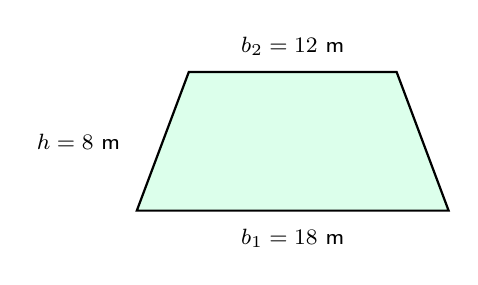
\begin{tikzpicture}[scale=0.22]
						\draw[thick,fill=vallightgreen] (0,0)--(18,0)--(15,8)--(3,8)--cycle;
						\node[below] at (9,-0.5) {\footnotesize $b_1=18$ m};
						\node[above] at (9,8.4) {\footnotesize $b_2=12$ m};
						\node[left] at (-0.4,4) {\footnotesize $h=8$ m};
					\end{tikzpicture}
				\end{center}
				a) Área del lote: $A=$\boxfill[2.6cm] m$^2$\\
				b) Rollos necesarios: \boxfill[2.4cm]
				
				\item \textbf{Carpintería.} Se construye el tablero triangular de una mesa. Un litro de barniz alcanza para $0,5$ m$^2$.
				\begin{center}
					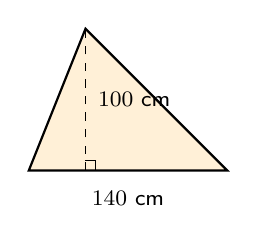
\begin{tikzpicture}[scale=0.018]
						\draw[thick,fill=vallightorange] (0,0)--(140,0)--(40,100)--cycle;
						\draw[dashed] (40,0)--(40,100);
						\draw (40,7)--(47,7)--(47,0);
						\node[below] at (70,-8) {\footnotesize $140$ cm};
						\node[right] at (42,50) {\footnotesize $100$ cm};
					\end{tikzpicture}
				\end{center}
				a) Área en cm$^2$: \boxfill[2.6cm] $=$ \boxfill[2cm] m$^2$\\
				b) Litros de barniz que se deben \textbf{comprar} (redondea hacia arriba): \boxfill[2.2cm]
				
				\item \textbf{Paisajismo.} Un parque triangular se rodea con una cerca, y se ubica un poste de luz cada $6$ metros (incluyendo el inicio).
				\begin{center}
					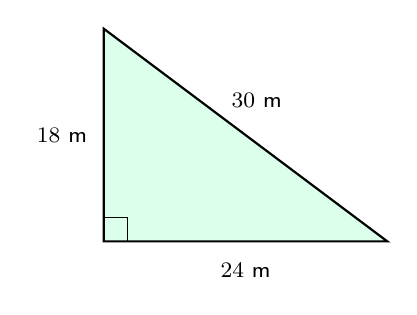
\begin{tikzpicture}[scale=0.15]
						\draw[thick,fill=vallightgreen] (0,0)--(24,0)--(0,18)--cycle;
						\draw (0,2)--(2,2)--(2,0);
						\node[below] at (12,-1) {\footnotesize $24$ m};
						\node[left] at (-0.6,9) {\footnotesize $18$ m};
						\node[above right] at (10,10.5) {\footnotesize $30$ m};
					\end{tikzpicture}
				\end{center}
				a) Perímetro: $P=$\boxfill[2.6cm] m\\
				b) Número de postes necesarios: \boxfill[2.2cm]
				
				\item \textbf{Jardinería (figura compuesta).} La planta de un cobertizo tiene forma de ``casa'': un rectángulo con un triángulo encima. Halla el área \textbf{total}.
				\begin{center}
					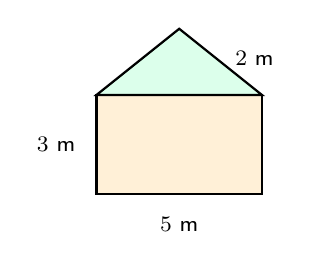
\begin{tikzpicture}[scale=0.42]
						\draw[thick,fill=vallightorange] (0,0) rectangle (5,3);
						\draw[thick,fill=vallightgreen] (0,3)--(5,3)--(2.5,5)--cycle;
						\node[below] at (2.5,-0.4) {\footnotesize $5$ m};
						\node[left] at (-0.35,1.5) {\footnotesize $3$ m};
						\node[right] at (3.9,4.1) {\footnotesize $2$ m};
					\end{tikzpicture}
				\end{center}
				a) Área del rectángulo: \boxfill[2cm]\\
				b) Área del triángulo: \boxfill[2cm]\\
				c) Área \textbf{total} del cobertizo: \boxfill[2.6cm]
				
				\item \textbf{Carpintería.} Una terraza de madera trapezoidal se cubre con tablas; cada tabla cubre $0,75$ m$^2$ y cuesta \$32.000.
				\begin{center}
					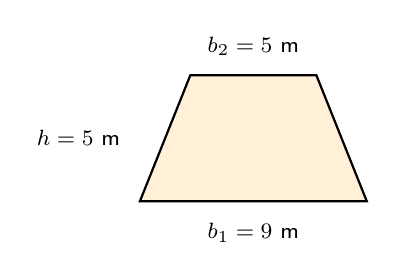
\begin{tikzpicture}[scale=0.32]
						\draw[thick,fill=vallightorange] (0,0)--(9,0)--(7,5)--(2,5)--cycle;
						\node[below] at (4.5,-0.5) {\footnotesize $b_1=9$ m};
						\node[above] at (4.5,5.4) {\footnotesize $b_2=5$ m};
						\node[left] at (-0.4,2.5) {\footnotesize $h=5$ m};
					\end{tikzpicture}
				\end{center}
				a) Área: $A=$\boxfill[2.4cm] m$^2$\quad b) Tablas necesarias: \boxfill[2.2cm]\\
				c) Costo total de la madera: \boxfill[3cm]
			\end{enumerate}
		\end{multicols}
		
		\vspace{0.3cm}
		\textbf{C) Polígonos regulares (perímetro $P=n\times s$, área $A=\dfrac{P\times a}{2}$).}
		
		\begin{multicols}{2}
			\begin{enumerate}[label=\textbf{\arabic*.}, itemsep=0.8cm, start=16]
				\item Pentágono regular ($n=5$).
				\begin{center}
					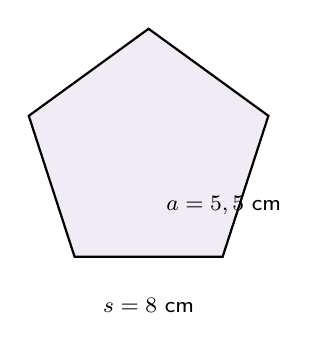
\begin{tikzpicture}[scale=0.5]
						\foreach \i in {0,...,4}{\coordinate (R\i) at ({90+72*\i}:3.2);}
						\draw[thick,fill=valpurple!10] (R0)--(R1)--(R2)--(R3)--(R4)--cycle;
						\node[below] at (0,-3.4) {\footnotesize $s=8$ cm};
						\node[right] at (0.2,-1.3) {\footnotesize $a=5,5$ cm};
					\end{tikzpicture}
				\end{center}
				$P=\boxfill[0.6cm]\times\boxfill[0.6cm]=$\boxfill[1.3cm]\\
				$A=\dfrac{\boxfill[1cm]\times\boxfill[0.8cm]}{\boxfill[0.5cm]}=$\boxfill[1.3cm]
				
				\item Hexágono regular ($n=6$).
				\begin{center}
					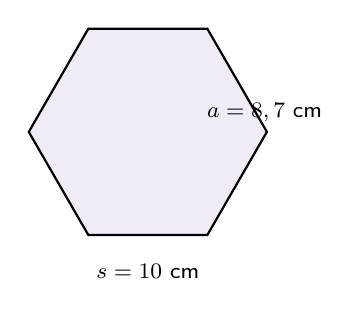
\begin{tikzpicture}[scale=0.42]
						\foreach \i in {0,...,5}{\coordinate (S\i) at ({60*\i}:3.6);}
						\draw[thick,fill=valpurple!10] (S0)--(S1)--(S2)--(S3)--(S4)--(S5)--cycle;
						\node[below] at (0,-3.7) {\footnotesize $s=10$ cm};
						\node[right] at (1.5,0.6) {\footnotesize $a=8,7$ cm};
					\end{tikzpicture}
				\end{center}
				$P=\boxfill[0.6cm]\times\boxfill[0.6cm]=$\boxfill[1.3cm]\\
				$A=\dfrac{\boxfill[1cm]\times\boxfill[0.8cm]}{\boxfill[0.5cm]}=$\boxfill[1.3cm]
				
				\item Cuadrado visto como polígono regular ($n=4$). Al final, compara tu resultado con la fórmula conocida $A=\text{lado}^2$.
				\begin{center}
					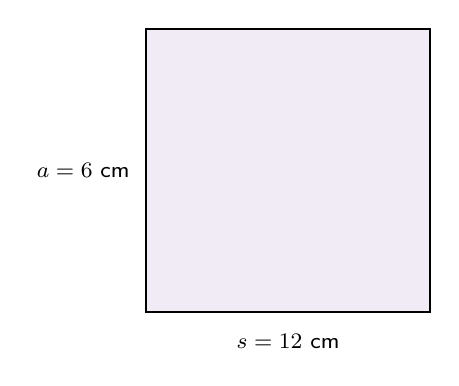
\begin{tikzpicture}[scale=0.3]
						\draw[thick,fill=valpurple!10] (0,0) rectangle (12,12);
						\node[below] at (6,-0.5) {\footnotesize $s=12$ cm};
						\node[left] at (-0.3,6) {\footnotesize $a=6$ cm};
					\end{tikzpicture}
				\end{center}
				$P=$\boxfill[1.6cm] \qquad $A=$\boxfill[1.6cm]\\
				¿Coincide con $12^2$? \boxfill[1.2cm]
				
				\item Octágono regular ($n=8$).
				\begin{center}
					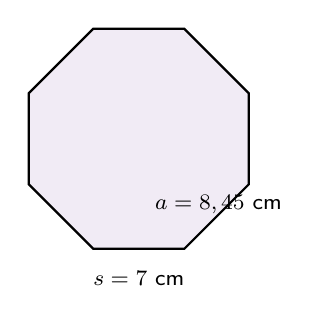
\begin{tikzpicture}[scale=0.42]
						\foreach \i in {0,...,7}{\coordinate (T\i) at ({22.5+45*\i}:3.6);}
						\draw[thick,fill=valpurple!10] (T0)--(T1)--(T2)--(T3)--(T4)--(T5)--(T6)--(T7)--cycle;
						\node[below] at (0,-3.7) {\footnotesize $s=7$ cm};
						\node[right] at (0.2,-2) {\footnotesize $a=8,45$ cm};
					\end{tikzpicture}
				\end{center}
				$P=\boxfill[0.6cm]\times\boxfill[0.6cm]=$\boxfill[1.3cm]\\
				$A=\dfrac{\boxfill[1cm]\times\boxfill[0.8cm]}{\boxfill[0.5cm]}=$\boxfill[1.3cm]
				
				\item Heptágono regular ($n=7$).
				\begin{center}
					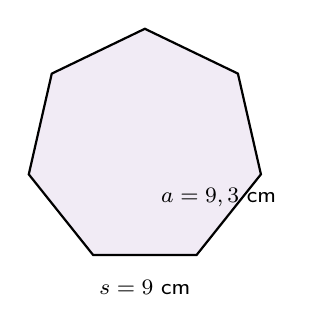
\begin{tikzpicture}[scale=0.42]
						\foreach \i in {0,...,6}{\coordinate (U\i) at ({90+51.43*\i}:3.6);}
						\draw[thick,fill=valpurple!10] (U0)--(U1)--(U2)--(U3)--(U4)--(U5)--(U6)--cycle;
						\node[below] at (0,-3.7) {\footnotesize $s=9$ cm};
						\node[right] at (0.2,-1.5) {\footnotesize $a=9,3$ cm};
					\end{tikzpicture}
				\end{center}
				$P=\boxfill[0.6cm]\times\boxfill[0.6cm]=$\boxfill[1.3cm]\\
				$A=\dfrac{\boxfill[1cm]\times\boxfill[0.8cm]}{\boxfill[0.5cm]}=$\boxfill[1.3cm]
				
				\item \textbf{Carpintería.} Una mesa hexagonal de jardín tiene lado $s=40$ cm y apotema $a=34,6$ cm. Se le pondrá un vidrio protector que cuesta \$0,50 por cm$^2$.
				\begin{center}
					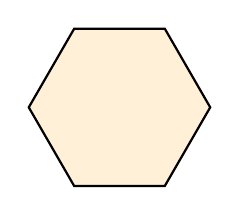
\begin{tikzpicture}[scale=0.32]
						\foreach \i in {0,...,5}{\coordinate (V\i) at ({60*\i}:3.6);}
						\draw[thick,fill=vallightorange] (V0)--(V1)--(V2)--(V3)--(V4)--(V5)--cycle;
					\end{tikzpicture}
				\end{center}
				a) Área: \boxfill[2.6cm] cm$^2$ \quad b) Costo del vidrio: \boxfill[3cm]
				
				\item \textbf{Paisajismo.} Una fuente octagonal mide $s=2$ m y $a=2,4$ m. Se quiere poner un borde decorativo alrededor.
				\begin{center}
					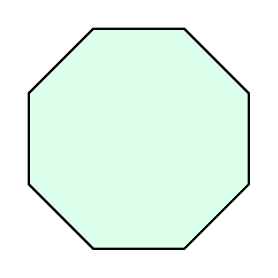
\begin{tikzpicture}[scale=0.42]
						\foreach \i in {0,...,7}{\coordinate (W\i) at ({22.5+45*\i}:3.6);}
						\draw[thick,fill=vallightgreen] (W0)--(W1)--(W2)--(W3)--(W4)--(W5)--(W6)--(W7)--cycle;
					\end{tikzpicture}
				\end{center}
				Perímetro del borde decorativo: $P=$\boxfill[3cm]
				
				\item \textbf{Reto (razonamiento inverso).} Un polígono regular tiene área $A=150$ cm$^2$ y apotema $a=10$ cm.
				\begin{enumerate}[label=\alph*)]
					\item Despeja $P$ de $A=\dfrac{P\times a}{2}$ y halla el perímetro: \boxfill[3cm]
					\item Si el polígono tiene $n=5$ lados, ¿cuánto mide cada lado $s$? \boxfill[2.4cm]
				\end{enumerate}
			\end{enumerate}
		\end{multicols}
	\end{practica}
	
	% =========================================================
	%  MISIÓN 2 — RECTAS PARALELAS, PERPENDICULARES Y TRANSVERSALES
	% =========================================================
	\section*{Misión 2: Rectas Paralelas, Perpendiculares y Transversales}
	
	% Figura base reutilizable: dos rectas paralelas r, s cortadas por una transversal t,
	% con P = intersección con r, Q = intersección con s.
	\newcommand{\transversalBase}{%
		\draw[thick] (-2.8,1.6) -- (2.8,1.6) node[right] {$r$};
		\draw[thick] (-2.8,-1.6) -- (2.8,-1.6) node[right] {$s$};
		\draw[thick] (-3.0,-2.1) -- (1.4,2.3) node[above right] {$t$};
		\draw[thick] (2.1,1.5) -- (2.1,1.7);
		\draw[thick] (2.1,-1.7) -- (2.1,-1.5);
		\coordinate (P) at (0.7,1.6);
		\coordinate (Q) at (-2.5,-1.6);
	}
	\newcommand{\marcarAngulo}[4]{\draw[#4,thick] ($(#1)+(#2:0.4)$) arc (#2:#3:0.4);}
	
	\begin{concepto}{Rectas Paralelas ($\parallel$) y Perpendiculares ($\perp$)}
		\textbf{Rectas paralelas ($\parallel$):} están en el mismo plano, tienen la \textbf{misma dirección} y \textbf{nunca se cruzan} (la distancia entre ellas es siempre la misma). Se escribe $r \parallel s$.\\
		\textbf{Rectas perpendiculares ($\perp$):} se cruzan formando exactamente un ángulo de $90^\circ$. Se escribe $r \perp s$.\\
		\textbf{Recta transversal:} una recta que \textbf{cruza} a otras dos (o más) rectas, cada una en un punto distinto.
		
		\begin{center}
			\begin{tikzpicture}[scale=0.55]
				\draw[thick,valblue] (0,2) -- (5,2); \draw[thick,valblue] (0,0) -- (5,0);
				\node[below] at (2.5,-0.4) {\footnotesize $r\parallel s$};
				\draw[thick,valorange] (8,0) -- (8,2.5); \draw[thick,valorange] (7,1.6) -- (10,1.6);
				\draw (8,1.6)++(0.25,0)--++(0,0.25)--++(-0.25,0);
				\node[below] at (8.5,-0.4) {\footnotesize $r\perp s$};
			\end{tikzpicture}
		\end{center}
	\end{concepto}
	
	\begin{concepto}{Ángulos Formados por una Transversal}
		Cuando una transversal $t$ corta a \textbf{dos rectas paralelas} $r$ y $s$, se forman \textbf{8 ángulos}: 4 en cada intersección. Se numeran así:
		
		\begin{center}
			\begin{tikzpicture}[scale=1.05, font=\small]
				\transversalBase
				\node at (0.49,2.11) {$1$}; \node at (1.21,1.81) {$2$};
				\node at (0.91,1.09) {$3$}; \node at (0.19,1.39) {$4$};
				\node at (-2.71,-1.09) {$5$}; \node at (-1.99,-1.39) {$6$};
				\node at (-2.29,-2.11) {$7$}; \node at (-3.01,-1.81) {$8$};
			\end{tikzpicture}
		\end{center}
		
		\begin{itemize}
			\item \textbf{Internos} (entre $r$ y $s$): $3,4,5,6$. \quad \textbf{Externos} (fuera de $r$ y $s$): $1,2,7,8$.
			\item \textbf{Correspondientes} (misma posición en cada recta, \textbf{congruentes}): $(1,5)$, $(2,6)$, $(3,7)$, $(4,8)$.
			\item \textbf{Alternos internos} (internos, lados opuestos de $t$, \textbf{congruentes}): $(3,5)$, $(4,6)$.
			\item \textbf{Alternos externos} (externos, lados opuestos de $t$, \textbf{congruentes}): $(1,7)$, $(2,8)$.
			\item \textbf{Internos (conjugados) del mismo lado} (internos, mismo lado de $t$, \textbf{suplementarios}, suman $180^\circ$): $(3,6)$, $(4,5)$.
			\item \textbf{Opuestos por el vértice} (\textbf{congruentes}): $(1,3)$, $(2,4)$, $(5,7)$, $(6,8)$.
			\item \textbf{Par lineal} (adyacentes sobre la misma recta, \textbf{suplementarios}): $(1,2)$, $(2,3)$, $(3,4)$, $(4,1)$ y análogos en $5,6,7,8$.
		\end{itemize}
	\end{concepto}
	
	\begin{ejemplo}
		\textbf{Situación:} en la figura anterior, $\angle 3 = 70^\circ$. Halla $\angle 5$, $\angle 6$ y $\angle 1$.
		\begin{center}
			\begin{tikzpicture}[scale=0.85, font=\small]
				\transversalBase
				\marcarAngulo{P}{225}{360}{valred}
				\node at (0.91,1.09) {\small $\angle 3{=}70^\circ$};
				\marcarAngulo{Q}{45}{180}{valgreen}
				\node at (-2.71,-1.09) {\small $\angle 5{=}?$};
			\end{tikzpicture}
		\end{center}
		$\angle 5$ es \textbf{alterno interno} con $\angle 3$ $\Rightarrow$ $\angle 5=70^\circ$ (congruentes).\\
		$\angle 6$ es \textbf{par lineal} con $\angle 5$ (suplementarios) $\Rightarrow$ $\angle 6=180^\circ-70^\circ=110^\circ$.\\
		$\angle 1$ es \textbf{correspondiente} con $\angle 5$ $\Rightarrow$ $\angle 1=70^\circ$ (congruentes).
	\end{ejemplo}
	
	\begin{truco}{Solo Dos Valores Posibles}
		En esta figura, \textbf{todos} los ángulos agudos son iguales entre sí, y \textbf{todos} los ángulos obtusos son iguales entre sí (si $t$ no es perpendicular a $r$ y $s$). Además, cualquier ángulo agudo + cualquier ángulo obtuso $=180^\circ$. Si conoces \textbf{uno solo} de los 8 ángulos, ¡puedes hallar los otros 7 sin usar transportador!
	\end{truco}
	
	\begin{minicheck}
		Usa la figura de esta misión: si $\angle 4 = 115^\circ$, halla $\angle 6$ (alternos internos): \boxfill[1.5cm]\quad y $\angle 8$ (opuestos por el vértice): \boxfill[1.5cm]
	\end{minicheck}
	
	\begin{practica}{Identificación de Ángulos entre Paralelas}
		
		\textbf{Usa la figura de referencia (arriba) para responder. Escribe el nombre de la relación o el valor pedido.}
		
		\begin{multicols}{2}
			\begin{enumerate}[label=\textbf{\arabic*.}, itemsep=0.75cm]
				\item Clasifica el par $\angle 1$ y $\angle 5$: \boxfill[2.8cm]
				\item Clasifica el par $\angle 3$ y $\angle 5$: \boxfill[2.8cm]
				\item Clasifica el par $\angle 2$ y $\angle 8$: \boxfill[2.8cm]
				\item Clasifica el par $\angle 4$ y $\angle 6$: \boxfill[2.8cm]
				\item Clasifica el par $\angle 3$ y $\angle 6$: \boxfill[2.8cm]
				\item Clasifica el par $\angle 1$ y $\angle 2$: \boxfill[2.8cm]
				\item Clasifica el par $\angle 2$ y $\angle 4$: \boxfill[2.8cm]
				\item ¿Cuál ángulo es \textbf{correspondiente} con $\angle 3$? \boxfill[2cm]
				\item ¿Cuál ángulo es \textbf{alterno interno} con $\angle 4$? \boxfill[2cm]
				\item Si $\angle 1=65^\circ$, halla $\angle 5$ (indica la relación usada): \boxfill[2.4cm]
				\item Si $\angle 4=70^\circ$, halla $\angle 2$ (indica la relación usada): \boxfill[2.4cm]
				\item Si $\angle 3=110^\circ$, halla $\angle 5$ (indica la relación usada): \boxfill[2.4cm]
				\item Si $\angle 2=75^\circ$, halla $\angle 7$ (indica la relación usada): \boxfill[2.4cm]
				
				\item Esta figura tiene la transversal inclinada hacia el \textbf{otro lado}. Clasifica $\angle 1$ y $\angle 8$:
				\begin{center}
					\begin{tikzpicture}[scale=0.75, font=\small]
						\begin{scope}[xscale=-1]
							\transversalBase
							\node at (0.49,2.11) {$1$}; \node at (1.21,1.81) {$2$};
							\node at (0.91,1.09) {$3$}; \node at (0.19,1.39) {$4$};
							\node at (-2.71,-1.09) {$5$}; \node at (-1.99,-1.39) {$6$};
							\node at (-2.29,-2.11) {$7$}; \node at (-3.01,-1.81) {$8$};
						\end{scope}
					\end{tikzpicture}
				\end{center}
				\boxfill[3.5cm]
				
				\item En la \textbf{misma} figura espejada del punto anterior: si $\angle 6=95^\circ$, halla $\angle 3$ (indica la relación usada): \boxfill[2.6cm]
			\end{enumerate}
		\end{multicols}
	\end{practica}
	
	% =========================================================
	%  MISIÓN 3 — CALCULANDO ÁNGULOS OCULTOS (ÁLGEBRA Y GEOMETRÍA)
	% =========================================================
	\section*{Misión 3: Calculando Ángulos Ocultos (Álgebra y Geometría)}
	
	\begin{concepto}{De la Relación Geométrica a la Ecuación}
		Cuando dos ángulos entre paralelas están expresados con \textbf{álgebra} (ej. $3x+20^\circ$), el primer paso es identificar \textbf{qué relación} los une:
		
		\begin{itemize}
			\item Si son \textbf{correspondientes}, \textbf{alternos internos}, \textbf{alternos externos} u \textbf{opuestos por el vértice} $\rightarrow$ son \textbf{congruentes}: se igualan las dos expresiones.
			\item Si son \textbf{par lineal} o \textbf{internos del mismo lado} (conjugados) $\rightarrow$ son \textbf{suplementarios}: la suma de las dos expresiones se iguala a $180^\circ$.
		\end{itemize}
	\end{concepto}
	
	\begin{ejemploresuelto}{Plantear y Resolver la Ecuación}
		\textbf{Situación:} $\angle 3=(3x+20)^\circ$ y $\angle 5=(5x-40)^\circ$.
		\begin{center}
			\begin{tikzpicture}[scale=0.85, font=\small]
				\transversalBase
				\marcarAngulo{P}{225}{360}{valred}
				\node at (0.91,1.09) {\scriptsize $3x{+}20^\circ$};
				\marcarAngulo{Q}{45}{180}{valgreen}
				\node at (-2.71,-1.09) {\scriptsize $5x{-}40^\circ$};
			\end{tikzpicture}
		\end{center}
		\begin{pasocaja}{valblue}{1}{Identificar la relación}
			\centering $\angle 3$ y $\angle 5$ son \textbf{alternos internos} $\Rightarrow$ son \textbf{congruentes}.
		\end{pasocaja}
		\begin{pasocaja}{valgreen}{2}{Plantear la ecuación}
			\centering $3x+20 = 5x-40$
		\end{pasocaja}
		\begin{pasocaja}{valorange}{3}{Resolver}
			\centering $20+40=5x-3x \;\Rightarrow\; 60=2x \;\Rightarrow\; x=30$
		\end{pasocaja}
		\begin{pasocaja}{valdark}{4}{Verificar con el enunciado original}
			\centering $\angle 3=3(30)+20=110^\circ \qquad \angle 5=5(30)-40=110^\circ$ \checkmark
		\end{pasocaja}
	\end{ejemploresuelto}
	
	\begin{errorcomun}{Igualar cuando debía ser suma $180^\circ$}
		\textbf{Incorrecto:} tratar un par lineal o conjugado interno como si fueran congruentes.\\
		\textbf{Correcto:} primero clasifica la pareja (¿congruente o suplementaria?) y \textbf{después} escribe la ecuación.
	\end{errorcomun}
	
	\begin{practica}{Álgebra y Geometría: Halla el valor de $x$}
		
		\textbf{Identifica la relación entre los ángulos marcados, plantea la ecuación en el espacio dado y resuelve.}
		
		\begin{multicols}{2}
			\begin{enumerate}[label=\textbf{\arabic*.}, itemsep=1cm]
				\item Alternos internos.
				\begin{center}
					\begin{tikzpicture}[scale=0.62, font=\small]
						\transversalBase
						\marcarAngulo{P}{225}{360}{valred} \node at (0.91,1.09) {\scriptsize $3x{+}10^\circ$};
						\marcarAngulo{Q}{45}{180}{valgreen} \node at (-2.71,-1.09) {\scriptsize $5x{-}38^\circ$};
					\end{tikzpicture}
				\end{center}
				Ecuación: \boxfill[4cm] \quad $x=$\boxfill[1.5cm]
				
				\item Correspondientes.
				\begin{center}
					\begin{tikzpicture}[scale=0.62, font=\small]
						\transversalBase
						\marcarAngulo{P}{0}{45}{valred} \node at (1.21,1.81) {\scriptsize $6x{-}5^\circ$};
						\marcarAngulo{Q}{0}{45}{valgreen} \node at (-1.99,-1.39) {\scriptsize $4x{+}27^\circ$};
					\end{tikzpicture}
				\end{center}
				Ecuación: \boxfill[4cm] \quad $x=$\boxfill[1.5cm]
				
				\item Par lineal.
				\begin{center}
					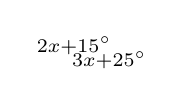
\begin{tikzpicture}[scale=0.62, font=\small]
						\transversalBase
						\marcarAngulo{P}{45}{180}{valred} \node at (0.49,2.11) {\scriptsize $2x{+}15^\circ$};
						\marcarAngulo{P}{0}{45}{valgreen} \node at (1.21,1.81) {\scriptsize $3x{+}25^\circ$};
					\end{tikzpicture}
				\end{center}
				Ecuación: \boxfill[4cm] \quad $x=$\boxfill[1.5cm]
				
				\item Alternos externos.
				\begin{center}
					\begin{tikzpicture}[scale=0.62, font=\small]
						\transversalBase
						\marcarAngulo{P}{45}{180}{valred} \node at (0.49,2.11) {\scriptsize $8x{-}12^\circ$};
						\marcarAngulo{Q}{225}{360}{valgreen} \node at (-2.29,-2.11) {\scriptsize $6x{+}18^\circ$};
					\end{tikzpicture}
				\end{center}
				Ecuación: \boxfill[4cm] \quad $x=$\boxfill[1.5cm]
				
				\item Internos del mismo lado (conjugados).
				\begin{center}
					\begin{tikzpicture}[scale=0.62, font=\small]
						\transversalBase
						\marcarAngulo{P}{180}{225}{valred} \node at (0.19,1.39) {\scriptsize $4x{+}25^\circ$};
						\marcarAngulo{Q}{45}{180}{valgreen} \node at (-2.71,-1.09) {\scriptsize $2x{+}35^\circ$};
					\end{tikzpicture}
				\end{center}
				Ecuación: \boxfill[4cm] \quad $x=$\boxfill[1.5cm]
				
				\item Opuestos por el vértice.
				\begin{center}
					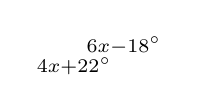
\begin{tikzpicture}[scale=0.62, font=\small]
						\transversalBase
						\marcarAngulo{P}{0}{45}{valred} \node at (1.21,1.81) {\scriptsize $6x{-}18^\circ$};
						\marcarAngulo{P}{180}{225}{valgreen} \node at (0.19,1.39) {\scriptsize $4x{+}22^\circ$};
					\end{tikzpicture}
				\end{center}
				Ecuación: \boxfill[4cm] \quad $x=$\boxfill[1.5cm]
				
				\item Alternos internos.
				\begin{center}
					\begin{tikzpicture}[scale=0.62, font=\small]
						\transversalBase
						\marcarAngulo{P}{180}{225}{valred} \node at (0.19,1.39) {\scriptsize $2x{+}30^\circ$};
						\marcarAngulo{Q}{0}{45}{valgreen} \node at (-1.99,-1.39) {\scriptsize $5x{-}15^\circ$};
					\end{tikzpicture}
				\end{center}
				Ecuación: \boxfill[4cm] \quad $x=$\boxfill[1.5cm]
				
				\item Correspondientes.
				\begin{center}
					\begin{tikzpicture}[scale=0.62, font=\small]
						\transversalBase
						\marcarAngulo{P}{225}{360}{valred} \node at (0.91,1.09) {\scriptsize $5x{-}10^\circ$};
						\marcarAngulo{Q}{225}{360}{valgreen} \node at (-2.29,-2.11) {\scriptsize $3x{+}24^\circ$};
					\end{tikzpicture}
				\end{center}
				Ecuación: \boxfill[4cm] \quad $x=$\boxfill[1.5cm]
				
				\item Par lineal.
				\begin{center}
					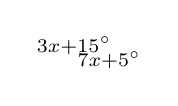
\begin{tikzpicture}[scale=0.62, font=\small]
						\transversalBase
						\marcarAngulo{P}{225}{360}{valred} \node at (0.91,1.09) {\scriptsize $7x{+}5^\circ$};
						\marcarAngulo{P}{180}{225}{valgreen} \node at (0.19,1.39) {\scriptsize $3x{+}15^\circ$};
					\end{tikzpicture}
				\end{center}
				Ecuación: \boxfill[4cm] \quad $x=$\boxfill[1.5cm]
				
				\item Internos del mismo lado (conjugados).
				\begin{center}
					\begin{tikzpicture}[scale=0.62, font=\small]
						\transversalBase
						\marcarAngulo{P}{225}{360}{valred} \node at (0.91,1.09) {\scriptsize $4x{+}20^\circ$};
						\marcarAngulo{Q}{0}{45}{valgreen} \node at (-1.99,-1.39) {\scriptsize $2x{+}40^\circ$};
					\end{tikzpicture}
				\end{center}
				Ecuación: \boxfill[4cm] \quad $x=$\boxfill[1.5cm]
				
				\item Alternos externos.
				\begin{center}
					\begin{tikzpicture}[scale=0.62, font=\small]
						\transversalBase
						\marcarAngulo{P}{0}{45}{valred} \node at (1.21,1.81) {\scriptsize $3x{+}40^\circ$};
						\marcarAngulo{Q}{180}{225}{valgreen} \node at (-3.01,-1.81) {\scriptsize $5x{+}10^\circ$};
					\end{tikzpicture}
				\end{center}
				Ecuación: \boxfill[4cm] \quad $x=$\boxfill[1.5cm]
				
				\item Opuestos por el vértice.
				\begin{center}
					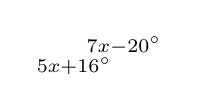
\begin{tikzpicture}[scale=0.62, font=\small]
						\transversalBase
						\marcarAngulo{Q}{0}{45}{valred} \node at (-1.99,-1.39) {\scriptsize $7x{-}20^\circ$};
						\marcarAngulo{Q}{180}{225}{valgreen} \node at (-3.01,-1.81) {\scriptsize $5x{+}16^\circ$};
					\end{tikzpicture}
				\end{center}
				Ecuación: \boxfill[4cm] \quad $x=$\boxfill[1.5cm]
				
				\item Correspondientes.
				\begin{center}
					\begin{tikzpicture}[scale=0.62, font=\small]
						\transversalBase
						\marcarAngulo{P}{45}{180}{valred} \node at (0.49,2.11) {\scriptsize $9x{-}30^\circ$};
						\marcarAngulo{Q}{45}{180}{valgreen} \node at (-2.71,-1.09) {\scriptsize $5x{+}18^\circ$};
					\end{tikzpicture}
				\end{center}
				Ecuación: \boxfill[4cm] \quad $x=$\boxfill[1.5cm]
				
				\item Par lineal.
				\begin{center}
					\begin{tikzpicture}[scale=0.62, font=\small]
						\transversalBase
						\marcarAngulo{Q}{225}{360}{valred} \node at (-2.29,-2.11) {\scriptsize $3x{+}35^\circ$};
						\marcarAngulo{Q}{180}{225}{valgreen} \node at (-3.01,-1.81) {\scriptsize $2x{+}25^\circ$};
					\end{tikzpicture}
				\end{center}
				Ecuación: \boxfill[4cm] \quad $x=$\boxfill[1.5cm]
				
				\item \textbf{Reto:} alternos externos. Después de hallar $x$, calcula también $\angle 4$ (usa una segunda relación).
				\begin{center}
					\begin{tikzpicture}[scale=0.62, font=\small]
						\transversalBase
						\marcarAngulo{P}{45}{180}{valred} \node at (0.49,2.11) {\scriptsize $6x{+}15^\circ$};
						\marcarAngulo{Q}{225}{360}{valgreen} \node at (-2.29,-2.11) {\scriptsize $4x{+}45^\circ$};
					\end{tikzpicture}
				\end{center}
				Ecuación: \boxfill[4cm] \quad $x=$\boxfill[1.5cm] \quad $\angle 4=$\boxfill[1.8cm]
			\end{enumerate}
		\end{multicols}
	\end{practica}
	
	% =========================================================
	%  MISIÓN 4 — TRANSFORMACIONES GEOMÉTRICAS
	% =========================================================
	\section*{Misión 4: Transformaciones Geométricas}
	
	\newcommand{\planoCart}[4]{%
		\draw[gray!25,thin] (#1,#3) grid (#2,#4);
		\draw[thick,-{Stealth}] (#1,0) -- ({#2+0.5},0) node[right,font=\scriptsize] {$x$};
		\draw[thick,-{Stealth}] (0,#3) -- (0,{#4+0.5}) node[above,font=\scriptsize] {$y$};
	}
	
	\begin{concepto}{Traslación}
		Una \textbf{traslación} desliza \textbf{todos} los puntos de una figura la \textbf{misma distancia} y en la \textbf{misma dirección}, sin girar ni voltear. Si el vector de traslación es $(a,b)$:
		$$(x,y) \;\longrightarrow\; (x+a,\;y+b)$$
		\begin{center}
			\begin{tikzpicture}[scale=0.55]
				\planoCart{-1}{7}{-1}{6}
				\draw[thick,fill=valblue!20] (1,1)--(4,1)--(2,3)--cycle;
				\draw[thick,fill=valorange!25] (4,-2)--(7,-2)--(5,0)--cycle;
				\draw[valdark,dashed,-{Stealth}] (2,3)--(5,0);
				\node[valblue,font=\scriptsize] at (2,1.4) {$ABC$};
				\node[valorange,font=\scriptsize] at (5,-1.6) {$A'B'C'$};
			\end{tikzpicture}
		\end{center}
	\end{concepto}
	
	\begin{concepto}{Reflexión}
		Una \textbf{reflexión} voltea la figura como un espejo sobre un \textbf{eje}. La figura y su imagen quedan a la \textbf{misma distancia} del eje, en lados opuestos.
		$$\text{Eje } x:\;(x,y)\to(x,-y) \qquad \text{Eje } y:\;(x,y)\to(-x,y) \qquad \text{Recta } y{=}x:\;(x,y)\to(y,x)$$
		\begin{center}
			\begin{tikzpicture}[scale=0.55]
				\planoCart{-5}{5}{-5}{5}
				\draw[thick,fill=valblue!20] (1,1)--(4,1)--(2,4)--cycle;
				\draw[thick,fill=valorange!25] (1,-1)--(4,-1)--(2,-4)--cycle;
				\node[valblue,font=\scriptsize] at (2,1.5) {$ABC$};
				\node[valorange,font=\scriptsize] at (2,-1.6) {$A'B'C'$};
			\end{tikzpicture}
		\end{center}
	\end{concepto}
	
	\begin{concepto}{Rotación}
		Una \textbf{rotación} gira la figura alrededor de un \textbf{centro} (aquí, siempre el origen) un cierto \textbf{ángulo} y \textbf{sentido}.
		$$90^\circ \text{ antihorario:}\;(x,y)\to(-y,x)$$
		$$180^\circ:\;(x,y)\to(-x,-y)$$
		$$90^\circ \text{ horario:}\;(x,y)\to(y,-x)$$
		\begin{center}
			\begin{tikzpicture}[scale=0.55]
				\planoCart{-5}{5}{-1}{5}
				\draw[thick,fill=valblue!20] (1,1)--(4,1)--(2,3)--cycle;
				\draw[thick,fill=valorange!25] (-1,1)--(-1,4)--(-3,2)--cycle;
				\node[valblue,font=\scriptsize] at (2,1.6) {$ABC$};
				\node[valorange,font=\scriptsize] at (-1.6,2) {$A'B'C'$};
			\end{tikzpicture}
		\end{center}
	\end{concepto}
	
	\begin{truco}{Solo Cambia el Signo o el Orden}
		No memorices dibujos: memoriza qué le pasa a las \textbf{coordenadas}. Reflejar cambia \textbf{signos}; rotar $90^\circ$ \textbf{intercambia} $x$ y $y$ (con algún signo); trasladar \textbf{suma} un vector. Con la regla algebraica puedes resolver \textbf{sin dibujar}.
	\end{truco}
	
	\begin{minicheck}
		El punto $(3,-5)$ se refleja sobre el eje $y$. Nueva coordenada: \boxfill[2.4cm]\\
		El punto $(2,6)$ se rota $180^\circ$ sobre el origen. Nueva coordenada: \boxfill[2.4cm]
	\end{minicheck}
	
	\begin{practica}{Transformaciones Geométricas}
		
		\begin{multicols}{2}
			\begin{enumerate}[label=\textbf{\arabic*.}, itemsep=1cm]
				\item \textbf{Traslación.} Dibuja la imagen de $ABC$ según el vector $(3,-4)$ y escribe sus coordenadas.
				\begin{center}
					\begin{tikzpicture}[scale=0.42]
						\planoCart{-1}{8}{-5}{5}
						\draw[thick,fill=valblue!20] (1,1)--(4,1)--(2,3)--cycle;
						\node[font=\scriptsize] at (0.6,0.6) {$A$}; \node[font=\scriptsize] at (4.3,0.7) {$B$}; \node[font=\scriptsize] at (2,3.4) {$C$};
					\end{tikzpicture}
				\end{center}
				$A'($\boxfill[0.9cm]$,$\boxfill[0.9cm]$)$ \quad $B'($\boxfill[0.9cm]$,$\boxfill[0.9cm]$)$ \quad $C'($\boxfill[0.9cm]$,$\boxfill[0.9cm]$)$
				
				\item \textbf{Reflexión sobre el eje $x$.} Dibuja la imagen y escribe sus coordenadas.
				\begin{center}
					\begin{tikzpicture}[scale=0.42]
						\planoCart{-1}{7}{-6}{6}
						\draw[thick,fill=valblue!20] (2,2)--(5,2)--(3,5)--cycle;
						\node[font=\scriptsize] at (1.6,1.6) {$A$}; \node[font=\scriptsize] at (5.3,1.7) {$B$}; \node[font=\scriptsize] at (3,5.4) {$C$};
					\end{tikzpicture}
				\end{center}
				$A'($\boxfill[0.9cm]$,$\boxfill[0.9cm]$)$ \quad $B'($\boxfill[0.9cm]$,$\boxfill[0.9cm]$)$ \quad $C'($\boxfill[0.9cm]$,$\boxfill[0.9cm]$)$
				
				\item \textbf{Reflexión sobre el eje $y$.} Dibuja la imagen y escribe sus coordenadas.
				\begin{center}
					\begin{tikzpicture}[scale=0.42]
						\planoCart{-6}{6}{-1}{6}
						\draw[thick,fill=valblue!20] (-4,1)--(-1,1)--(-2,4)--cycle;
						\node[font=\scriptsize] at (-4.4,0.7) {$A$}; \node[font=\scriptsize] at (-0.6,0.7) {$B$}; \node[font=\scriptsize] at (-2,4.4) {$C$};
					\end{tikzpicture}
				\end{center}
				$A'($\boxfill[0.9cm]$,$\boxfill[0.9cm]$)$ \quad $B'($\boxfill[0.9cm]$,$\boxfill[0.9cm]$)$ \quad $C'($\boxfill[0.9cm]$,$\boxfill[0.9cm]$)$
				
				\item \textbf{Rotación $90^\circ$ antihoraria} sobre el origen. Dibuja la imagen y escribe sus coordenadas.
				\begin{center}
					\begin{tikzpicture}[scale=0.42]
						\planoCart{-6}{6}{-1}{6}
						\draw[thick,fill=valblue!20] (2,1)--(5,1)--(3,4)--cycle;
						\node[font=\scriptsize] at (1.6,0.7) {$A$}; \node[font=\scriptsize] at (5.3,0.7) {$B$}; \node[font=\scriptsize] at (3,4.4) {$C$};
					\end{tikzpicture}
				\end{center}
				$A'($\boxfill[0.9cm]$,$\boxfill[0.9cm]$)$ \quad $B'($\boxfill[0.9cm]$,$\boxfill[0.9cm]$)$ \quad $C'($\boxfill[0.9cm]$,$\boxfill[0.9cm]$)$
				
				\item \textbf{Rotación $180^\circ$} sobre el origen (cuadrado $ABCD$). Dibuja la imagen y escribe sus coordenadas.
				\begin{center}
					\begin{tikzpicture}[scale=0.42]
						\planoCart{-5}{5}{-5}{5}
						\draw[thick,fill=valblue!20] (1,1) rectangle (3,3);
						\node[font=\scriptsize] at (0.6,0.7) {$A$}; \node[font=\scriptsize] at (3.4,0.7) {$B$};
						\node[font=\scriptsize] at (3.4,3.3) {$C$}; \node[font=\scriptsize] at (0.6,3.3) {$D$};
					\end{tikzpicture}
				\end{center}
				$A'($\boxfill[0.9cm]$,$\boxfill[0.9cm]$)$ \; $B'($\boxfill[0.9cm]$,$\boxfill[0.9cm]$)$ \; $C'($\boxfill[0.9cm]$,$\boxfill[0.9cm]$)$ \; $D'($\boxfill[0.9cm]$,$\boxfill[0.9cm]$)$
				
				\item \textbf{Rotación $90^\circ$ horaria} sobre el origen. Dibuja la imagen y escribe sus coordenadas.
				\begin{center}
					\begin{tikzpicture}[scale=0.42]
						\planoCart{-1}{6}{-6}{5}
						\draw[thick,fill=valblue!20] (2,1)--(5,1)--(3,3)--cycle;
						\node[font=\scriptsize] at (1.6,0.7) {$A$}; \node[font=\scriptsize] at (5.3,0.7) {$B$}; \node[font=\scriptsize] at (3,3.4) {$C$};
					\end{tikzpicture}
				\end{center}
				$A'($\boxfill[0.9cm]$,$\boxfill[0.9cm]$)$ \quad $B'($\boxfill[0.9cm]$,$\boxfill[0.9cm]$)$ \quad $C'($\boxfill[0.9cm]$,$\boxfill[0.9cm]$)$
				
				\item \textbf{Identifica la transformación} (nombre + vector, eje, o ángulo y sentido).
				\begin{center}
					\begin{tikzpicture}[scale=0.4]
						\planoCart{-2}{6}{-6}{6}
						\draw[thick,fill=valblue!20] (1,1)--(3,1)--(1,4)--cycle;
						\draw[thick,fill=valorange!25] (1,-1)--(3,-1)--(1,-4)--cycle;
					\end{tikzpicture}
				\end{center}
				\boxfill[5cm]
				
				\item \textbf{Identifica la transformación.}
				\begin{center}
					\begin{tikzpicture}[scale=0.4]
						\planoCart{-6}{6}{-1}{6}
						\draw[thick,fill=valblue!20] (2,2)--(5,2)--(2,5)--cycle;
						\draw[thick,fill=valorange!25] (-2,2)--(-5,2)--(-2,5)--cycle;
					\end{tikzpicture}
				\end{center}
				\boxfill[5cm]
				
				\item \textbf{Identifica la transformación} (halla también el vector exacto).
				\begin{center}
					\begin{tikzpicture}[scale=0.4]
						\planoCart{-1}{8}{-1}{8}
						\draw[thick,fill=valblue!20] (1,1)--(4,1)--(2,3)--cycle;
						\draw[thick,fill=valorange!25] (3,4)--(6,4)--(4,6)--cycle;
					\end{tikzpicture}
				\end{center}
				\boxfill[5cm]
				
				\item \textbf{Identifica la transformación.}
				\begin{center}
					\begin{tikzpicture}[scale=0.4]
						\planoCart{-6}{6}{-1}{6}
						\draw[thick,fill=valblue!20] (3,1)--(3,4)--(1,1)--cycle;
						\draw[thick,fill=valorange!25] (-1,3)--(-4,3)--(-1,1)--cycle;
					\end{tikzpicture}
				\end{center}
				\boxfill[5cm]
				
				\item \textbf{Identifica la transformación.}
				\begin{center}
					\begin{tikzpicture}[scale=0.4]
						\planoCart{-5}{5}{-5}{5}
						\draw[thick,fill=valblue!20] (1,1)--(4,1)--(2,4)--cycle;
						\draw[thick,fill=valorange!25] (-1,-1)--(-4,-1)--(-2,-4)--cycle;
					\end{tikzpicture}
				\end{center}
				\boxfill[5cm]
				
				\item \textbf{Solo álgebra (sin dibujar).} El punto $P(4,-2)$ se refleja sobre la recta $y=x$.
				\begin{center}
					\begin{tikzpicture}[scale=0.42]
						\planoCart{-4}{5}{-4}{5}
						\fill[valblue] (4,-2) circle (2.5pt); \node[right,font=\scriptsize] at (4.1,-2) {$P(4,-2)$};
					\end{tikzpicture}
				\end{center}
				$P'=($\boxfill[1cm]$,$\boxfill[1cm]$)$
				
				\item \textbf{Solo álgebra (sin dibujar).} El punto $Q(-3,5)$ se rota $90^\circ$ en sentido \textbf{horario} sobre el origen.
				\begin{center}
					\begin{tikzpicture}[scale=0.42]
						\planoCart{-5}{6}{-1}{6}
						\fill[valblue] (-3,5) circle (2.5pt); \node[above,font=\scriptsize] at (-3,5.2) {$Q(-3,5)$};
					\end{tikzpicture}
				\end{center}
				$Q'=($\boxfill[1cm]$,$\boxfill[1cm]$)$
				
				\item \textbf{Transformación compuesta (2 pasos).} Al triángulo $ABC$ se le aplica primero una reflexión sobre el eje $x$, y luego una traslación según $(2,3)$.
				\begin{center}
					\begin{tikzpicture}[scale=0.42]
						\planoCart{-1}{6}{-4}{4}
						\draw[thick,fill=valblue!20] (1,1)--(3,1)--(1,3)--cycle;
					\end{tikzpicture}
				\end{center}
				Paso 1 (reflexión): $A'($\boxfill[0.7cm]$,$\boxfill[0.7cm]$)$ $B'($\boxfill[0.7cm]$,$\boxfill[0.7cm]$)$ $C'($\boxfill[0.7cm]$,$\boxfill[0.7cm]$)$\\
				Paso 2 (traslación): $A''($\boxfill[0.7cm]$,$\boxfill[0.7cm]$)$ $B''($\boxfill[0.7cm]$,$\boxfill[0.7cm]$)$ $C''($\boxfill[0.7cm]$,$\boxfill[0.7cm]$)$
				
				\item \textbf{Reto de discriminación.} ¿Rotación o reflexión? Identifica con precisión.
				\begin{center}
					\begin{tikzpicture}[scale=0.4]
						\planoCart{-1}{7}{-1}{7}
						\draw[thick,fill=valblue!20] (1,3)--(4,3)--(1,5)--cycle;
						\draw[thick,fill=valorange!25] (3,1)--(3,4)--(5,1)--cycle;
					\end{tikzpicture}
				\end{center}
				\boxfill[5cm]
			\end{enumerate}
		\end{multicols}
	\end{practica}
	
\end{document}